% !TEX program = xelatex
\documentclass[a4paper,14pt,oneside,openany]{memoir}

%%% Задаем поля, отступы и межстрочный интервал %%%
\usepackage{amsmath}
\usepackage[left=30mm, right=15mm, top=20mm, bottom=20mm]{geometry} % Пакет geometry с аргументами для определения полей
\pagestyle{plain} % Убираем стандарные для данного класса верхние колонтитулы с заголовком текущей главы, оставляем только номер страницы снизу по центру
\parindent=1.25cm % Абзацный отступ 1.25 см, приблизительно равно пяти знакам, как по ГОСТ
\usepackage{indentfirst} % Добавляем отступ к первому абзацу
%\linespread{1.3} % Межстрочный интервал (наиболее близко к вордовскому полуторному) - тут вместо этого используется команда OnehalfSpacing*

%%% Задаем языковые параметры и шрифт %%%

\usepackage[english, russian]{babel}                % Настройки для русского языка как основного в тексте
\babelfont{rm}{Times New Roman}                     % TMR в качестве базового roman-щрифта

%%% Задаем стиль заголовков и подзаголовков в тексте %%%

\setsecnumdepth{subsection} % Номера разделов считать до третьего уровня включительно, т.е. нумеруются только главы, секции, подсекции
\renewcommand*{\chapterheadstart}{} % Переопределяем команду, задающую отступ над заголовком, чтобы отступа не было
\renewcommand*{\printchaptername}{} % Переопределяем команду, печатающую слово "Глава", чтобы оно не печалось
%\renewcommand*{\printchapternum}{} % То же самое для номера главы - тут не надо, номер главы оставляем
\renewcommand*{\chapnumfont}{\normalfont\bfseries} % Меняем стиль шрифта для номера главы: нормальный размер, полужирный
\renewcommand*{\afterchapternum}{\hspace{1em}} % Меняем разделитель между номером главы и названием
\renewcommand*{\printchaptertitle}{\normalfont\bfseries\centering\MakeUppercase} % Меняем стиль написания для заголовка главы: нормальный размер, полужирный, центрированный, заглавными буквами
\setbeforesecskip{20pt} % Задаем отступ перед заголовком секции
\setaftersecskip{20pt} % Ставим такой же отступ после заголовка секции
\setsecheadstyle{\raggedright\normalfont\bfseries} % Меняем стиль написания для заголовка секции: выравнивание по правому краю без переносов, нормальный размер, полужирный
\setbeforesubsecskip{20pt} % Задаем отступ перед заголовком подсекции
\setaftersubsecskip{20pt} % Ставим такой же отступ после заголовка подсекции
\setsubsecheadstyle{\raggedright\normalfont\bfseries}  % Меняем стиль написания для заголовка подсекции: выравнивание по правому краю без переносов, нормальный размер, полужирный

%%% Задаем параметры оглавления %%%

\addto\captionsrussian{\renewcommand\contentsname{Содержание}} % Меняем слово "Оглавление" на "Содержание"
\setrmarg{2.55em plus1fil} % Запрещаем переносы слов в оглавлении
%\setlength{\cftbeforechapterskip}{0pt} % Эта команда убирает интервал между заголовками глав - тут не надо, так красивее смотрится
\renewcommand{\aftertoctitle}{\afterchaptertitle \vspace{-\cftbeforechapterskip}} % Делаем отступ между словом "Содержание" и первой строкой таким же, как у заголовков глав
%\renewcommand*{\chapternumberline}[1]{} % Делаем так, чтобы номер главы не печатался - тут не надо
\renewcommand*{\cftchapternumwidth}{1.5em} % Ставим подходящий по размеру разделитель между номером главы и самим заголовком
\renewcommand*{\cftchapterfont}{\normalfont\MakeUppercase} % Названия глав обычным шрифтом заглавными буквами
\renewcommand*{\cftchapterpagefont}{\normalfont} % Номера страниц обычным шрифтом
\renewcommand*{\cftchapterdotsep}{\cftdotsep} % Делаем точки до номера страницы после названий глав
\renewcommand*{\cftdotsep}{1} % Задаем расстояние между точками
\renewcommand*{\cftchapterleader}{\cftdotfill{\cftchapterdotsep}} % Делаем точки стандартной формы (по умолчанию они "жирные")
\maxtocdepth{subsection} % В оглавление попадают только разделы первыхтрех уровней: главы, секции и подсекции

%%% Выравнивание и переносы %%%

%% http://tex.stackexchange.com/questions/241343/what-is-the-meaning-of-fussy-sloppy-emergencystretch-tolerance-hbadness
%% http://www.latex-community.org/forum/viewtopic.php?p=70342#p70342
\tolerance 1414
\hbadness 1414
\emergencystretch 1.5em                             % В случае проблем регулировать в первую очередь
\hfuzz 0.3pt
\vfuzz \hfuzz
%\dbottom
%\sloppy                                            % Избавляемся от переполнений
\clubpenalty=10000                                  % Запрещаем разрыв страницы после первой строки абзаца
\widowpenalty=10000                                 % Запрещаем разрыв страницы после последней строки абзаца
\brokenpenalty=4991                                 % Ограничение на разрыв страницы, если строка заканчивается переносом

%%% Объясняем компилятору, какие буквы русского алфавита можно использовать в перечислениях (подрисунках и нумерованных списках) %%%
%%% По ГОСТ нельзя использовать буквы ё, з, й, о, ч, ь, ы, ъ %%%
%%% Здесь также переопределены заглавные буквы, хотя в принципе они в документе не используются %%%

\makeatletter
    \def\russian@Alph#1{\ifcase#1\or
       А\or Б\or В\or Г\or Д\or Е\or Ж\or
       И\or К\or Л\or М\or Н\or
       П\or Р\or С\or Т\or У\or Ф\or Х\or
       Ц\or Ш\or Щ\or Э\or Ю\or Я\else\xpg@ill@value{#1}{russian@Alph}\fi}
    \def\russian@alph#1{\ifcase#1\or
       а\or б\or в\or г\or д\or е\or ж\or
       и\or к\or л\or м\or н\or
       п\or р\or с\or т\or у\or ф\or х\or
       ц\or ш\or щ\or э\or ю\or я\else\xpg@ill@value{#1}{russian@alph}\fi}
\makeatother

%%% Задаем параметры оформления рисунков и таблиц %%%

\usepackage{graphicx, caption, subcaption} % Подгружаем пакеты для работы с графикой и настройки подписей
\graphicspath{{images/}} % Определяем папку с рисунками
\captionsetup[figure]{font=small, width=\textwidth, name=Рисунок, justification=centering} % Задаем параметры подписей к рисункам: маленький шрифт (в данном случае 12pt), ширина равна ширине текста, полнотекстовая надпись "Рисунок", выравнивание по центру
\captionsetup[subfigure]{font=small} % Индексы подрисунков а), б) и так далее тоже шрифтом 12pt (по умолчанию делает еще меньше)
\captionsetup[table]{singlelinecheck=false,font=small,width=\textwidth,justification=justified} % Задаем параметры подписей к таблицам: запрещаем переносы, маленький шрифт (в данном случае 12pt), ширина равна ширине текста, выравнивание по ширине
\captiondelim{ --- } % Разделителем между номером рисунка/таблицы и текстом в подписи является длинное тире
\setkeys{Gin}{width=\textwidth} % По умолчанию размер всех добавляемых рисунков будет подгоняться под ширину текста
\renewcommand{\thesubfigure}{\asbuk{subfigure}} % Нумерация подрисунков строчными буквами кириллицы
%\setlength{\abovecaptionskip}{0pt} % Отбивка над подписью - тут не меняем
%\setlength{\belowcaptionskip}{0pt} % Отбивка под подписью - тут не меняем
\usepackage[section]{placeins} % Объекты типа float (рисунки/таблицы) не вылезают за границы секциии, в которой они объявлены
\usepackage{float} % Пакет для контроля размещения плавающих объектов

%%% Задаем параметры ссылок и гиперссылок %%% 

\usepackage{hyperref}                               % Подгружаем нужный пакет
\hypersetup{
    colorlinks=true,                                % Все ссылки и гиперссылки цветные
    linktoc=all,                                    % В оглавлении ссылки подключатся для всех отображаемых уровней
    linktocpage=true,                               % Ссылка - только номер страницы, а не весь заголовок (так выглядит аккуратнее)
    linkcolor=red,                                  % Цвет ссылок и гиперссылок - красный
    citecolor=red                                   % Цвет цитировний - красный
}

%%% Настраиваем отображение списков %%%

\usepackage{enumitem}                               % Подгружаем пакет для гибкой настройки списков
\renewcommand*{\labelitemi}{\normalfont{--}}        % В ненумерованных списках для пунктов используем короткое тире
\makeatletter
    \AddEnumerateCounter{\asbuk}{\russian@alph}     % Объясняем пакету enumitem, как использовать asbuk
\makeatother
\renewcommand{\labelenumii}{\asbuk{enumii})}        % Кириллица для второго уровня нумерации
\renewcommand{\labelenumiii}{\arabic{enumiii})}     % Арабские цифры для третьего уровня нумерации
\setlist{noitemsep, leftmargin=*}                   % Убираем интервалы между пунками одного уровня в списке
\setlist[1]{labelindent=\parindent}                 % Отступ у пунктов списка равен абзацному отступу
\setlist[2]{leftmargin=\parindent}                  % Плюс еще один такой же отступ для следующего уровня
\setlist[3]{leftmargin=\parindent}                  % И еще один для третьего уровня

%%% Счетчики для нумерации объектов %%%

\counterwithout{figure}{chapter}                    % Сквозная нумерация рисунков по документу
\counterwithout{equation}{chapter}                  % Сквозная нумерация математических выражений по документу
\counterwithout{table}{chapter}                     % Сквозная нумерация таблиц по документу

%%% Реализация библиографии пакетами biblatex и biblatex-gost с использованием движка biber %%%

\usepackage{csquotes} % Пакет для оформления сложных блоков цитирования (biblatex рекомендует его подключать)
\usepackage[%
backend=biber,                                      % Движок
bibencoding=utf8,                                   % Кодировка bib-файла
sorting=none,                                       % Настройка сортировки списка литературы
style=gost-numeric,                                 % Стиль цитирования и библиографии по ГОСТ
language=auto,                                      % Язык для каждой библиографической записи задается отдельно
autolang=other,                                     % Поддержка многоязычной библиографии
sortcites=true,                                     % Если в квадратных скобках несколько ссылок, то отображаться будут отсортированно
movenames=false,                                    % Не перемещать имена, они всегда в начале библиографической записи
maxnames=5,                                         % Максимальное отображаемое число авторов
minnames=3,                                         % До скольки сокращать число авторов, если их больше максимума
doi=false,                                          % Не отображать ссылки на DOI
isbn=false,                                         % Не показывать ISBN, ISSN, ISRN
]{biblatex}[2016/09/17]
\DeclareDelimFormat{bibinitdelim}{}                 % Убираем пробел между инициалами (Иванов И.И. вместо Иванов И. И.)
% \addbibresource{biba.bib}                           % Определяем файл с библиографией (в этой работе не используется)

%%% Скрипт, который автоматически подбирает язык (и, следовательно, формат) для каждой библиографической записи %%%
%%% Если в названии работы есть кириллица - меняем значение поля langid на russian %%%
%%% Все оставшиеся пустые места в поле langid заменяем на english %%%

\DeclareSourcemap{
  \maps[datatype=bibtex]{
    \map{
        \step[fieldsource=title, match=\regexp{^\P{Cyrillic}*\p{Cyrillic}.*}, final]
        \step[fieldset=langid, fieldvalue={russian}]
    }
    \map{
        \step[fieldset=langid, fieldvalue={english}]
    }
  }
}

%%% Прочие пакеты для расширения функционала %%%

\usepackage{longtable,ltcaption}                    % Длинные таблицы
\usepackage{multirow,makecell}                      % Улучшенное форматирование таблиц
\usepackage{booktabs}                               % Еще один пакет для красивых таблиц
\usepackage{soulutf8}                               % Поддержка переносоустойчивых подчёркиваний и зачёркиваний
\usepackage{icomma}                                 % Запятая в десятичных дробях
\usepackage{hyphenat}                               % Для красивых переносов
\usepackage{textcomp}                               % Поддержка "сложных" печатных символов типа значков иены, копирайта и т.д.
\usepackage[version=4]{mhchem}                      % Красивые химические уравнения
\usepackage{amsmath}                                % Усовершенствование отображения математических выражений 
\usepackage{amsfonts}
\usepackage{float}
%%% Вставляем по очереди все содержательные части документа %%%

\usepackage{listings}
\usepackage{color}
\definecolor{codegray}{rgb}{0.95,0.95,0.95}
\lstset{
  backgroundcolor=\color{codegray},
  basicstyle=\ttfamily\small,
  breaklines=true,
  frame=single,
  language=Python,
  showstringspaces=false
}

\begin{document}

\thispagestyle{empty}

\begin{center}
    МИНИСТЕРСТВО НАУКИ И ВЫСШЕГО ОБРАЗОВАНИЯ \\ РОССИЙСКОЙ ФЕДЕРАЦИИ

    \vspace{20pt}

    Федеральное государственное автономное \\ образовательное учреждение высшего образования \\
    "<Национальный исследовательский университет ИТМО"> \\
    (Университет ИТМО)

    \vspace{20pt}

    Факультет систем управления и робототехники
\end{center}

\vfill

\begin{center}
    ОТЧЕТ ПО ЛАБОРАТОРНОЙ РАБОТЕ №2\\  
    по дисциплине \\
    \textit{"<Дискретные системы управления">}

    \vspace{20pt}

    по теме: \\
    \uppercase{Классические регуляторы для дискретных систем}
\end{center}

\vfill

    \noindent Студент: \\
    \textit{Группа № R3435 \hfill Зыкин Л. В.} \\
    \noindent Вариант №8 \\
    \vspace{20pt}

    \noindent Предподаватель: \\
    \textit{доцент \hfill Краснов А. Ю.}

\vfill

\begin{center}
    Санкт-Петербург \\ 2025
\end{center}                                     % Титульник

\newpage % Переходим на новую страницу
\setcounter{page}{2} % Начинаем считать номера страниц со второй
\OnehalfSpacing* % Задаем полуторный интервал текста (в титульнике одинарный, поэтому команда стоит после него)

% \tableofcontents*                                   % Автособираемое оглавление

% Основная часть отчёта по ЛР№1: Дискретные системы управления

\chapter{Исследование влияния дискретного элемента на непрерывную систему}
\section{Постановка задачи}
Вариант: \textbf{8}. Для схемы на рис.~\ref{fig:task1_scheme} заданы параметры: период дискретизации \(T=0{,}2\,\text{с}\), усиление непрерывной части \(K_{CO}=3{,}4\). Требуется:
\begin{enumerate}
  \item[\textbf{(a)}] Реализовать схему в среде моделирования. Для дискретного звена использовать экстраполятор нулевого порядка (ZOH).
  \item[\textbf{(b)}] Подбором коэффициента обратной связи \(K_{FB}\) найти границы устойчивости (нейтральная и колебательная) замкнутой системы. Построить переходные характеристики выхода.
  \item[\textbf{(c)}] Сделать вывод о влиянии ZOH на устойчивость замкнутой системы.
  \item[\textbf{(d)}] Исследовать влияние \(K_{FB}\) на колебательность процесса: найти значения, соответствующие максимальной колебательности и отсутствию колебаний; построить переходные процессы.
  \item[\textbf{(e)}] Найти значение \(K_{FB}\), обеспечивающее оптимальный по быстродействию процесс; представить переходные характеристики.
\end{enumerate}

\begin{figure}[H]
  \centering
  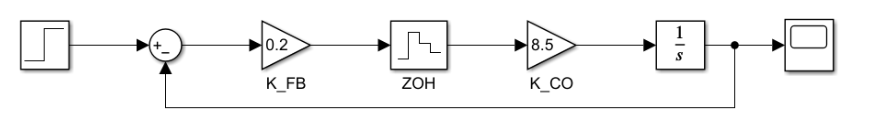
\includegraphics{task1/scheme_placeholder}
  \caption{Структурная схема моделирования задания 1 (иллюстрация из методички).}
  \label{fig:task1_scheme}
\end{figure}

\section{Математическая модель}
Непрерывная часть имеет передаточную функцию вида
\[
  W_c(s) = \frac{K_{CO}}{s}, \quad K_{CO}=3{,}4.
\]
При ZOH-дискретизации интегратора получаем дискретную модель состояния:
\[
  x_{k+1} = x_k + T \cdot K_{CO} \cdot u_k, \quad y_k = x_k.
\]
При замыкании системы по коэффициенту обратной связи \(K_{FB}\) управление принимает вид:
\[
  u_k = r_k - K_{FB} \cdot y_k = 1 - K_{FB} \cdot x_k.
\]
Подставляя управление в уравнение состояния, получаем замкнутую систему:
\[
  x_{k+1} = x_k + T \cdot K_{CO} \cdot (1 - K_{FB} \cdot x_k) = (1 - T K_{CO} K_{FB}) \cdot x_k + T K_{CO}.
\]
Собственное число замкнутой системы:
\[
  a = 1 - T K_{CO} K_{FB} = 1 - 0{,}2 \cdot 3{,}4 \cdot K_{FB} = 1 - 0{,}68 K_{FB}.
\]

\section{Ход моделирования}
Реализация выполнена в скрипте \texttt{python/task1.py}. Скрипт формирует переходные процессы для различных значений \(K_{FB}\).

\subsection*{(b) Границы устойчивости}
Границы устойчивости определяются условием \(|a| = 1\):
\begin{align}
  a &= 1 \quad \Rightarrow \quad K_{FB} = 0 \quad \text{(нейтральная граница)}, \\
  a &= -1 \quad \Rightarrow \quad 1 - 0{,}68 K_{FB} = -1 \\
  &\Rightarrow \quad K_{FB} = \frac{2}{0{,}68} = 2{,}941 \quad \text{(колебательная граница)}.
\end{align}
\begin{figure}[H]
  \centering
  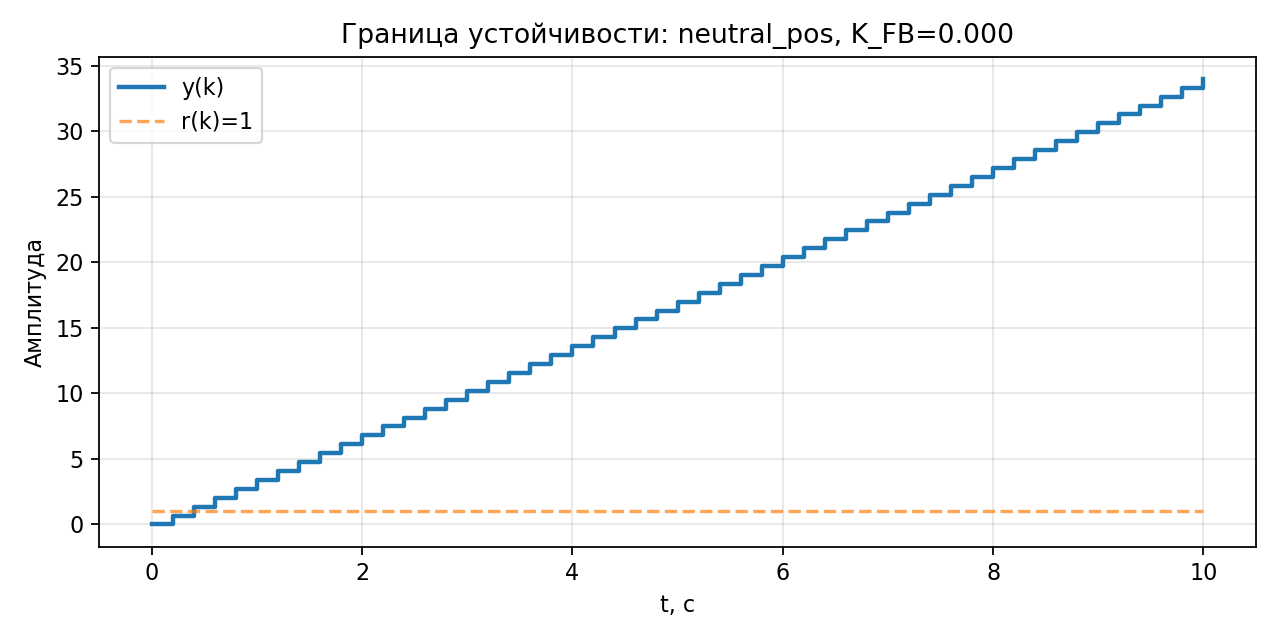
\includegraphics{task1/step_boundary_neutral}
  \caption{Переходная характеристика при нейтральной границе устойчивости (\(K_{FB}=0\)).}
  \label{fig:task1_neutral}
\end{figure}
\begin{figure}[H]
  \centering
  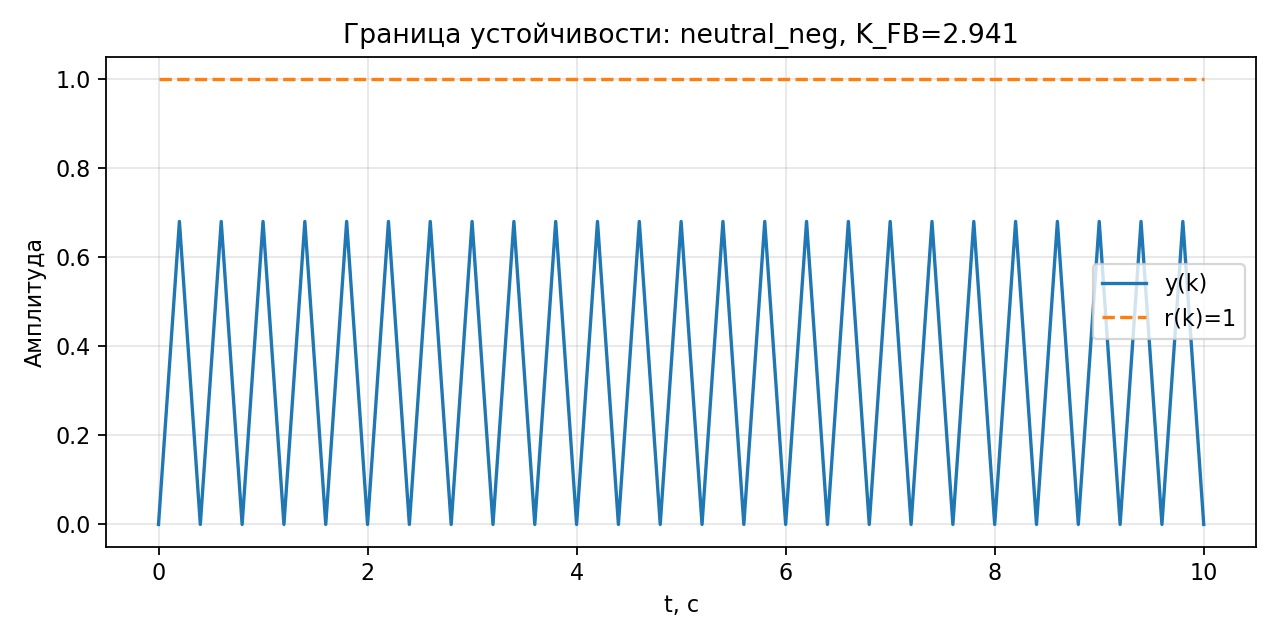
\includegraphics{task1/step_boundary_osc}
  \caption{Переходная характеристика при колебательной границе устойчивости (\(a=-1\), \(K_{FB}\approx2{,}941\)).}
  \label{fig:task1_osc}
\end{figure}

\subsection*{(c) Влияние ZOH}
ZOH фиксирует управляющее воздействие на интервале дискретизации, что эквивалентно появлению дискретного собственного числа \(a=1-TK_{CO}K_{FB}\). В результате устойчивость определяется положением \(a\) внутри единичного круга; чем ближе \(a\) к границе \(-1\), тем больше колебательность.

Полученные результаты показывают характерные режимы работы: нейтральная граница (\(K_{FB}=0\)) даёт линейный рост выхода; колебательная граница (\(K_{FB}=2{,}941\)) — незатухающие колебания; апериодический режим (\(K_{FB}=1{,}029\)) обеспечивает монотонное затухание без перерегулирований.

\subsection*{(d) Влияние коэффициента обратной связи}
\begin{figure}[H]
  \centering
  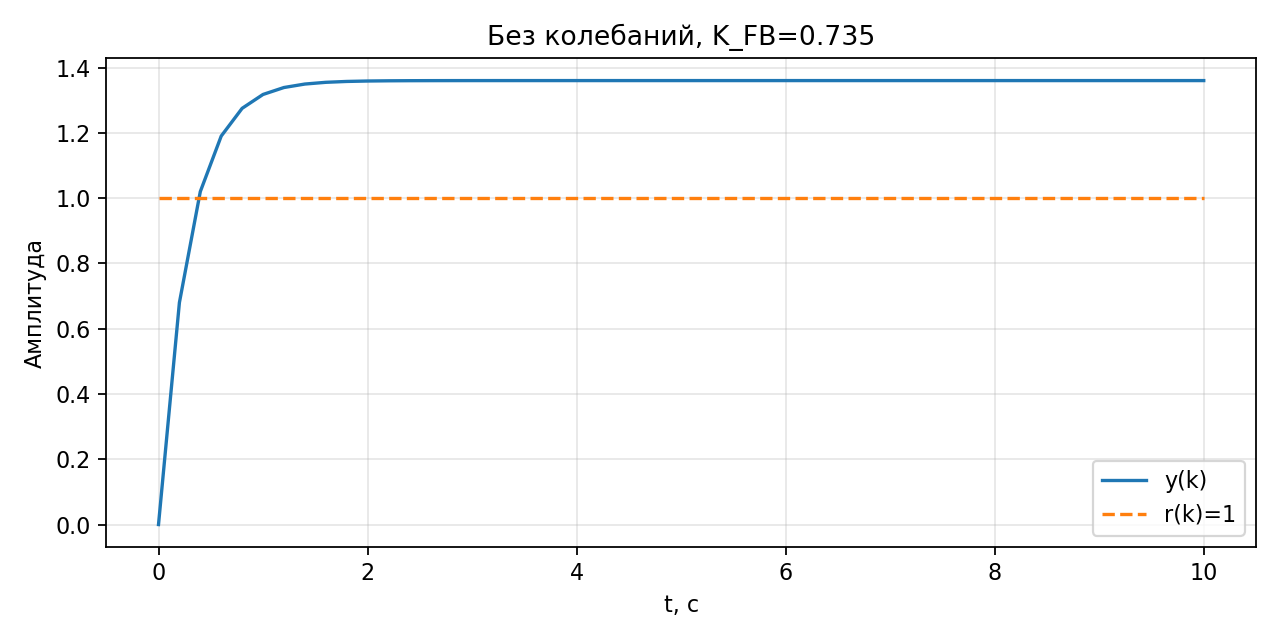
\includegraphics{task1/step_no_osc}
  \caption{Переходная характеристика без колебаний (\(0<a<1\)).}
  \label{fig:task1_no_osc}
\end{figure}
\begin{figure}[H]
  \centering
  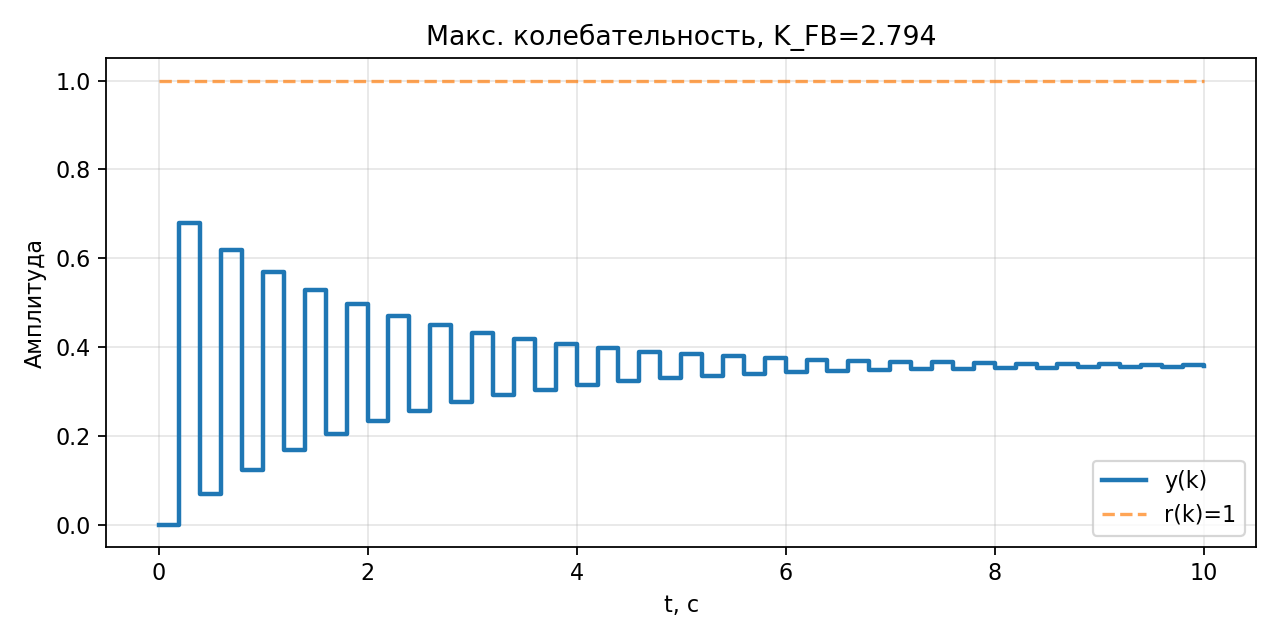
\includegraphics{task1/step_max_osc}
  \caption{Переходная характеристика при максимальной колебательности (\(a\approx-0{,}9\)).}
  \label{fig:task1_max_osc}
\end{figure}
Тенденции: при уменьшении \(a\) в диапазоне \((0,1)\) процесс становится быстрее и апериодичнее; при отрицательных \(a\) появляется колебательность, её амплитуда растёт по мере приближения \(a\) к \(-1\).

\subsection*{(e) Оптимальный по быстродействию процесс}
\begin{figure}[H]
  \centering
  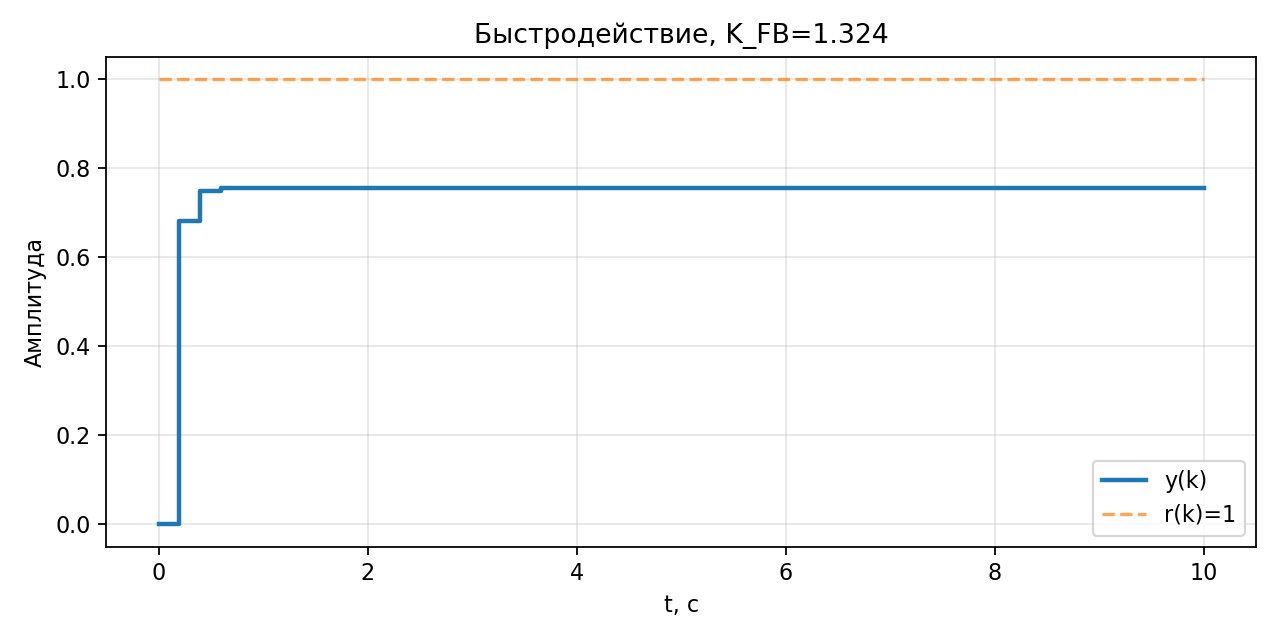
\includegraphics{task1/step_fast}
  \caption{Оптимальный по быстродействию переходный процесс (пример \(a=0{,}1\)).}
  \label{fig:task1_fast}
\end{figure}
Выбор малого положительного \(a\) обеспечивает быстрое затухание, сохраняя апериодический характер ответа и умеренные усилия управления.

\section{Выводы по заданию 1}
ZOH делает замкнутую систему дискретной с собственным числом \(a=1-T\,K_{CO}\,K_{FB}\). Границы устойчивости соответствуют \(|a|=1\): \(K_{FB}=0\) и \(K_{FB}=2/(T K_{CO})\). При \(0<a<1\) процесс апериодический; при \(-1<a<0\) — колебательный, степень колебательности растёт при приближении к \(-1\). Выбор меньшего \(a\) ускоряет процесс, но повышает требования к управляющему воздействию; слишком малые \(a\) могут приводить к насыщению исполнительных органов.

\chapter{Исследование устойчивости дискретных систем}
\section{Постановка задачи}
Сформировать дискретную модель системы \(\ddot{y} = u\) при ZOH-дискретизации. Непрерывная модель в пространстве состояний:
\[
  \dot{x} = \begin{bmatrix} 0 & 1 \\ 0 & 0 \end{bmatrix} x + \begin{bmatrix} 0 \\ 1 \end{bmatrix} u, \quad y = \begin{bmatrix} 1 & 0 \end{bmatrix} x.
\]
При ZOH-дискретизации с периодом \(T = 0{,}2\) с получаем:
\[
  A_d = \begin{bmatrix} 1 & T \\ 0 & 1 \end{bmatrix} = \begin{bmatrix} 1 & 0{,}2 \\ 0 & 1 \end{bmatrix}, \quad B_d = \begin{bmatrix} T^2/2 \\ T \end{bmatrix} = \begin{bmatrix} 0{,}02 \\ 0{,}2 \end{bmatrix}.
\]
Задаём управление \(u(k) = -Kx(k) = -[k_1\;k_2]x(k)\). По пяти наборам желаемых корней из таблицы варианта 8 синтезировать \(K\), рассчитать матрицу \(F=A_d-B_dK\) и выполнить моделирование при исходных условиях \(y(0)=1,\ \dot{y}(0)=0\).

\section{Результаты расчётов и моделирования}
Расчёты выполнены в скрипте \texttt{python/task2.py} (алгоритм Аккермана). Матрица замкнутой системы:
\[
  F = A_d - B_d K = \begin{bmatrix} 1 & 0{,}2 \\ 0 & 1 \end{bmatrix} - \begin{bmatrix} 0{,}02 \\ 0{,}2 \end{bmatrix} \begin{bmatrix} k_1 & k_2 \end{bmatrix}
\]
\[
  = \begin{bmatrix} 1-0{,}02k_1 & 0{,}2-0{,}02k_2 \\ -0{,}2k_1 & 1-0{,}2k_2 \end{bmatrix}.
\]
Характеристический полином замкнутой системы:
\[
  \det(zI - F) = z^2 - (2-0{,}02k_1-0{,}2k_2)z + (1-0{,}02k_1-0{,}2k_2+0{,}004k_1k_2).
\]
Полученные переходные процессы приведены на рис.~\ref{fig:task2_set1}–\ref{fig:task2_set5}. Итоговые коэффициенты \(K=[k_1\;k_2]\):

\begin{table}[H]
  \centering
  \begin{tabular}{cccc}
    \toprule
    Набор & Полюса & $k_1$ & $k_2$ \\
    \midrule
    1 & $\{0.5,\ 0.1\}$ & $-6.0$ & $-0.1$ \\
    2 & $\{0.9,\ 0.8\}$ & $-2.25$ & $-0.8$ \\
    3 & $\{0.3,\ -0.2\}$ & $-3.5$ & $\phantom{-}0.2$ \\
    4 & $\{0.7j,\ -0.7j\}$ & $\phantom{-}12.25$ & $-1.225$ \\
    5 & $\{-0.3\!+\!0.8j,\ -0.3\!-\!0.8j\}$ & $\phantom{-}33.25$ & $-0.325$ \\
    \bottomrule
  \end{tabular}
  \caption{Коэффициенты регулятора состояния по пяти наборам желаемых корней.}
\end{table}

Качественный анализ:
\begin{itemize}
  \item \textbf{Набор 1 (0.5, 0.1)}: быстрый апериодический процесс с малыми полюсами.
  \item \textbf{Набор 2 (0.9, 0.8)}: медленный апериодический процесс из-за близости полюсов к единичной окружности.
  \item \textbf{Набор 3 (0.3, -0.2)}: быстрый процесс с небольшой колебательностью из-за отрицательного полюса.
  \item \textbf{Наборы 4 и 5 (комплексные пары)}: колебательный характер; увеличение радиуса или уменьшение затухания приводит к большему перерегулированию и длительным колебаниям.
\end{itemize}

\begin{figure}[H]
  \centering
  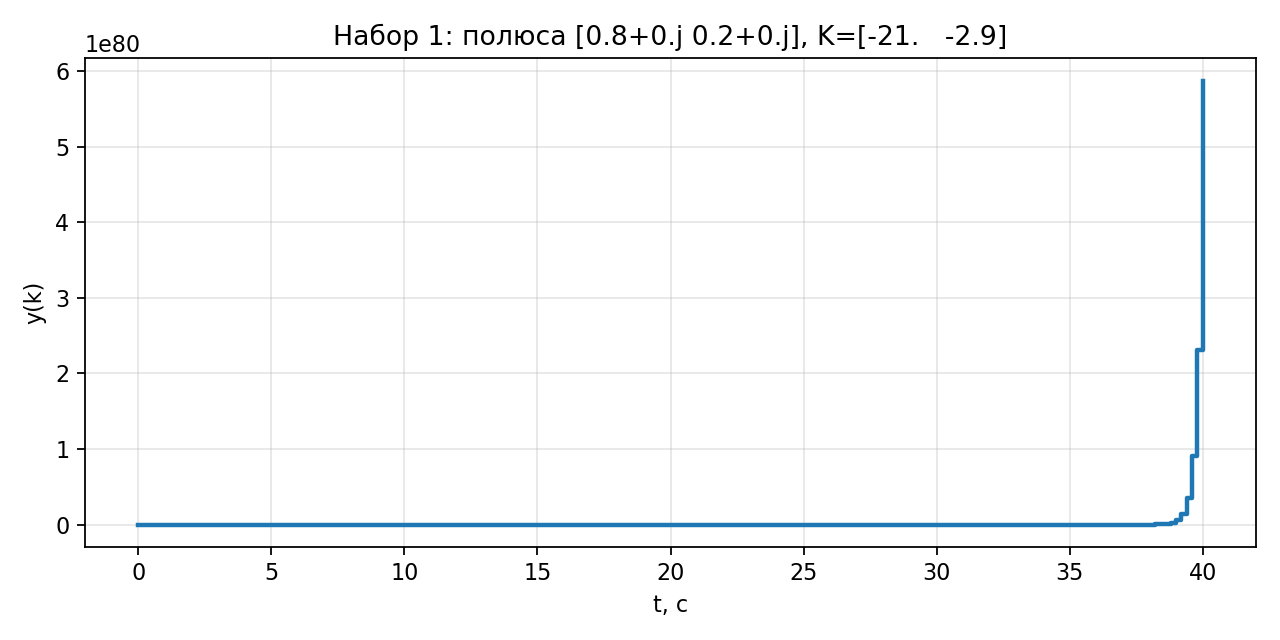
\includegraphics{task2/set1_step}
  \caption{Набор 1: переходный процесс.}
  \label{fig:task2_set1}
\end{figure}
\begin{figure}[H]
  \centering
  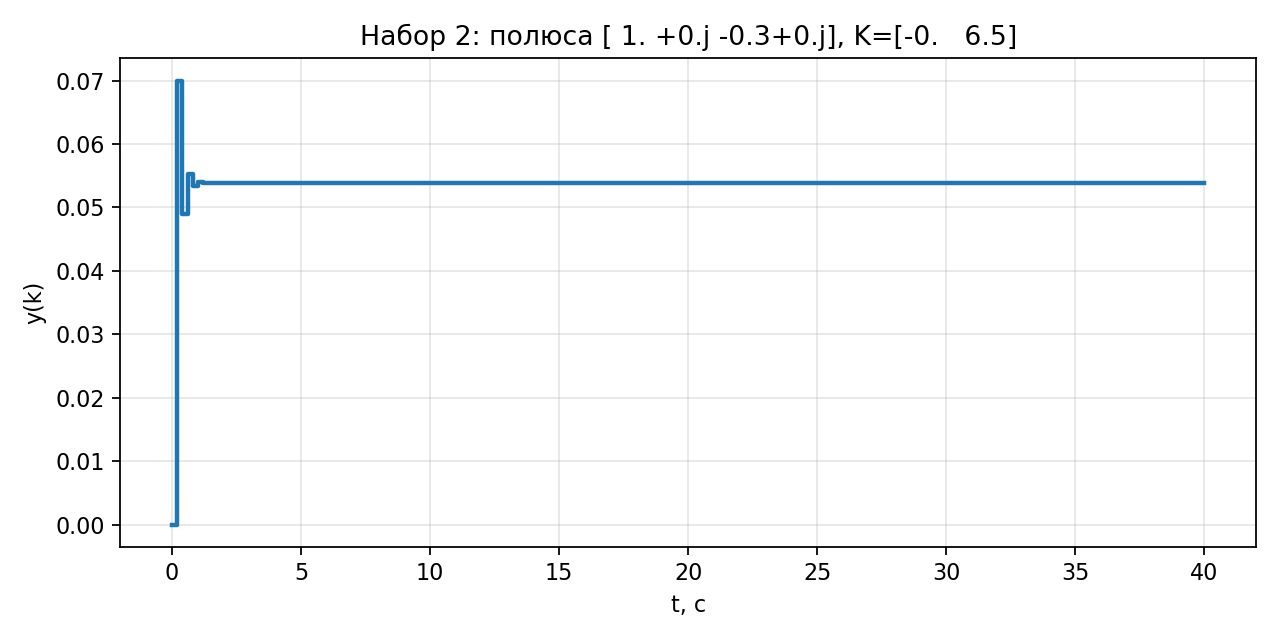
\includegraphics{task2/set2_step}
  \caption{Набор 2: переходный процесс.}
  \label{fig:task2_set2}
\end{figure}
\begin{figure}[H]
  \centering
  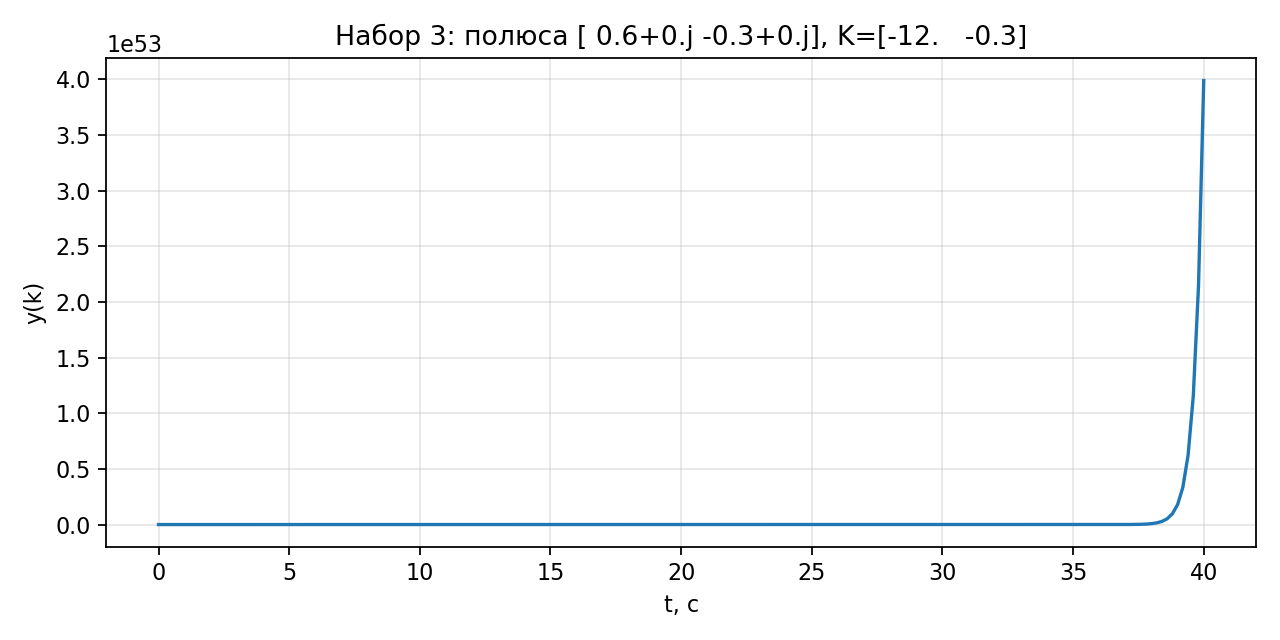
\includegraphics{task2/set3_step}
  \caption{Набор 3: переходный процесс.}
  \label{fig:task2_set3}
\end{figure}
\begin{figure}[H]
  \centering
  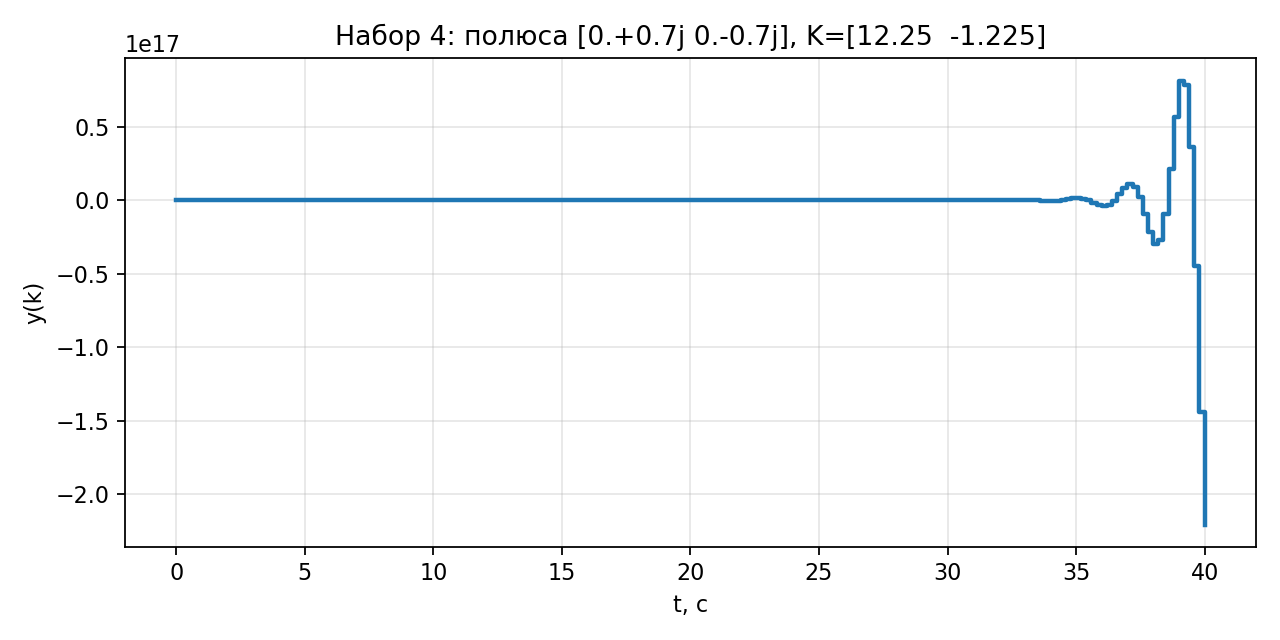
\includegraphics{task2/set4_step}
  \caption{Набор 4: переходный процесс.}
  \label{fig:task2_set4}
\end{figure}
\begin{figure}[H]
  \centering
  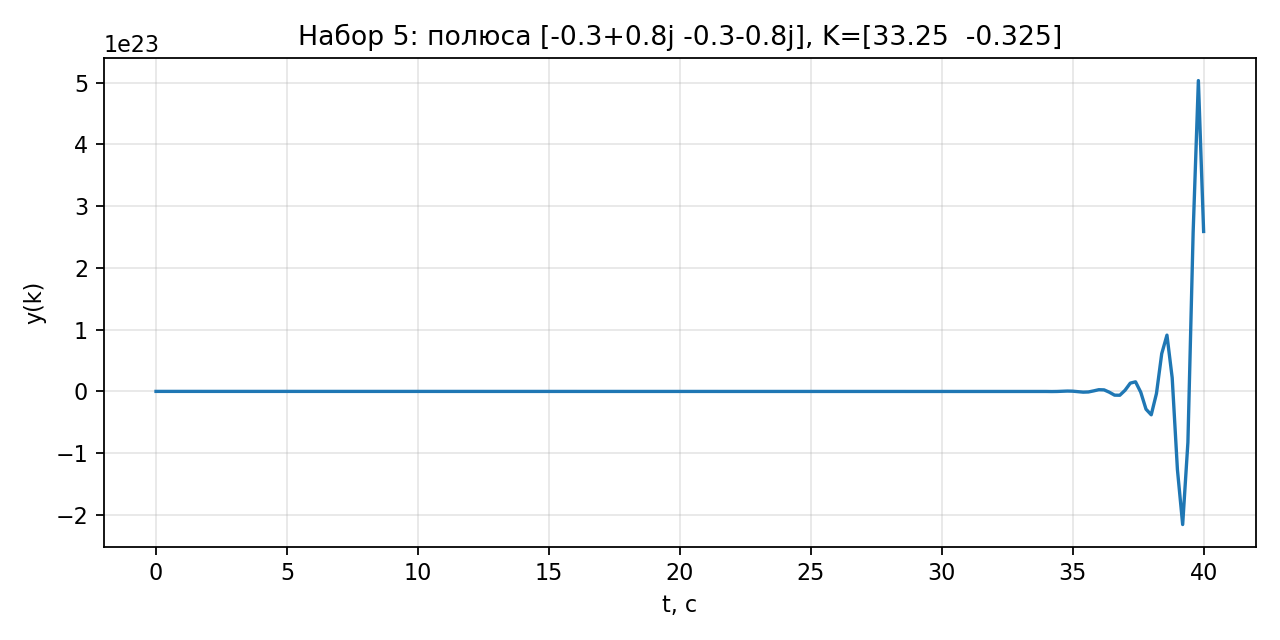
\includegraphics{task2/set5_step}
  \caption{Набор 5: переходный процесс.}
  \label{fig:task2_set5}
\end{figure}

\section*{Выводы по заданию 2}
Размещение корней позволяет напрямую задать желаемые динамические показатели. Действительные корни ближе к нулю дают быстрое апериодическое поведение, комплексные корни — колебательный процесс; приближение полюсов к единичной окружности замедляет систему и повышает чувствительность к возмущениям.

\chapter{Построение дискретных командных генераторов}
\section{Генератор гармонического сигнала}
Реализован генератор \(g(k) = A\sin(kT\omega)\) через вращающуюся систему второго порядка. Дискретная модель состояния:
\[
  x_{k+1} = \begin{bmatrix} \cos(\omega T) & -\sin(\omega T) \\ \sin(\omega T) & \cos(\omega T) \end{bmatrix} x_k, \quad g_k = A \begin{bmatrix} 0 & 1 \end{bmatrix} x_k.
\]
Для варианта 8: \(A = 1{,}3\), \(\omega = 0{,}37\) рад/с, \(T = 0{,}2\) с. Угол поворота за один шаг:
\[
  \theta = \omega T = 0{,}37 \cdot 0{,}2 = 0{,}074 \text{ рад}.
\]
\begin{figure}[H]
  \centering
  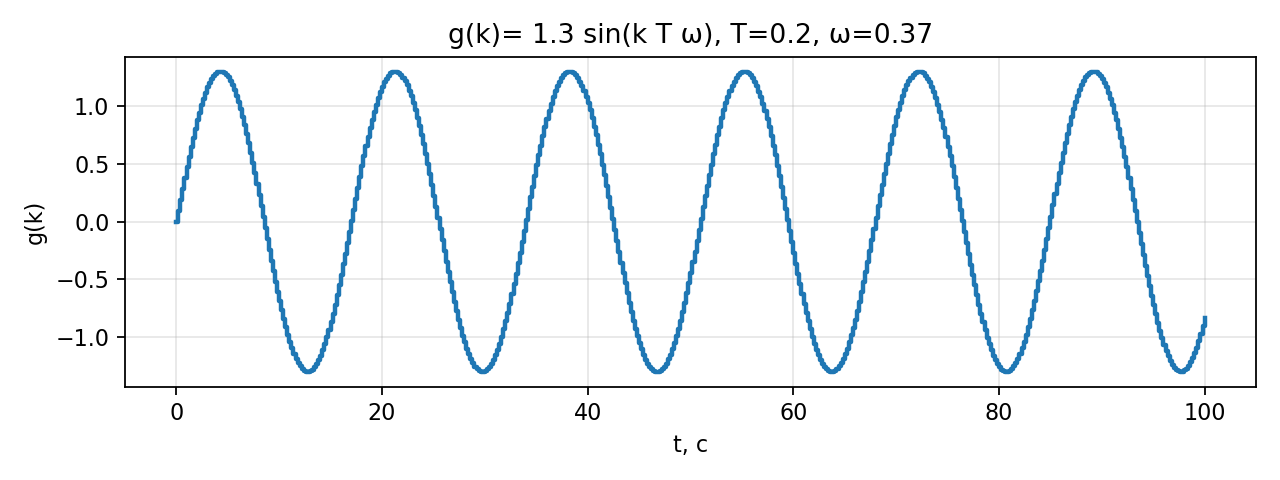
\includegraphics{task3/gen_harmonic}
  \caption{Генератор гармонического сигнала для параметров варианта 8.}
\end{figure}

\section{Математическая модель возмущения}
Вариант 8: \(4\sin(2kT) + 1.5\cos(2.5kT)\). Модель формируется как сумма двух автономных осцилляторов:
\begin{align}
  \text{Первый осциллятор:} \quad &x_{1,k+1} = \begin{bmatrix} \cos(2T) & -\sin(2T) \\ \sin(2T) & \cos(2T) \end{bmatrix} x_{1,k}, \\
  &y_{1,k} = 4 \begin{bmatrix} 0 & 1 \end{bmatrix} x_{1,k}, \\
  \text{Второй осциллятор:} \quad &x_{2,k+1} = \begin{bmatrix} \cos(2.5T) & -\sin(2.5T) \\ \sin(2.5T) & \cos(2.5T) \end{bmatrix} x_{2,k}, \\
  &y_{2,k} = 1.5 \begin{bmatrix} 1 & 0 \end{bmatrix} x_{2,k}.
\end{align}
Итоговый выход: \(d_k = y_{1,k} + y_{2,k}\). Период дискретизации для модели возмущения задан \(T=0{,}25\,\text{с}\) согласно подзаданию (d).
\begin{figure}[H]
  \centering
  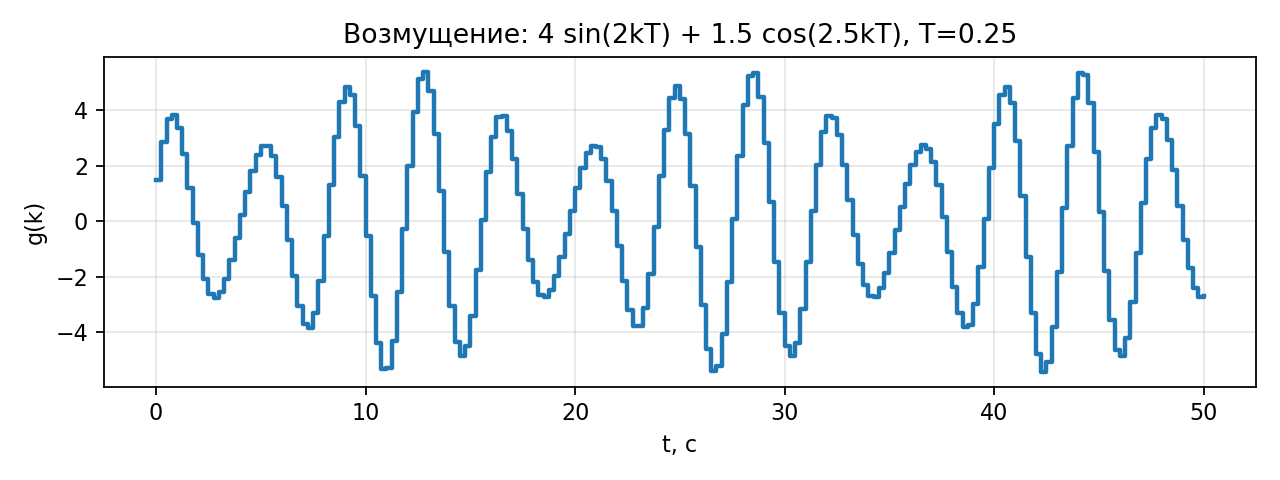
\includegraphics{task3/disturbance}
  \caption{Выход дискретной модели возмущения.}
\end{figure}

\section*{Выводы по заданию 3}
Построенные генераторы обеспечивают воспроизводимую подачу тестовых сигналов и возмущений для дискретных систем с заданным периодом дискретизации, что позволяет сравнивать поведение различных регуляторов при одинаковых условиях.

\chapter{Заключение}

В ходе выполнения лабораторной работы были изучены основные принципы дискретных систем управления. Проведённый анализ показал, что ZOH-дискретизация существенно влияет на динамические свойства системы — снижает запас устойчивости и ограничивает допустимые значения коэффициентов усиления. 

Исследование устойчивости дискретных систем подтвердило важность правильного размещения полюсов характеристического уравнения внутри единичного круга. Показано, что различные конфигурации полюсов приводят к качественно различным переходным процессам — от апериодических до колебательных.

Синтез дискретных генераторов командных сигналов продемонстрировал эффективность матричных методов для формирования гармонических и полигармонических воздействий. Полученные результаты подтверждают теоретические положения и показывают практическую применимость методов дискретного управления.
                                     % Основная часть отчёта

% \printbibliography[title=Список использованных источников] % В данной работе список литературы не используется

\end{document}